\documentclass[10pt]{beamer}
\usetheme[
%%% option passed to the outer theme
%    progressstyle=fixedCircCnt,   % fixedCircCnt, movingCircCnt (moving is deault)
  ]{Berlin}
  
% If you want to change the colors of the various elements in the theme, edit and uncomment the following lines

% Change the bar colors:
%\setbeamercolor{Feather}{fg=red!20,bg=red}

% Change the color of the structural elements:
%\setbeamercolor{structure}{fg=red}

% Change the frame title text color:
%\setbeamercolor{frametitle}{fg=blue}

% Change the normal text color background:
%\setbeamercolor{normal text}{fg=black,bg=gray!10}

%-------------------------------------------------------
% INCLUDE PACKAGES
%-------------------------------------------------------

\usepackage[utf8]{inputenc}
\usepackage[english]{babel}
\usepackage[T1]{fontenc}
\usepackage{amsmath}
\usepackage{helvet}
\usepackage{multirow}
\usepackage{graphicx}
\usepackage{comment}
\usepackage[absolute,overlay]{textpos}
\usepackage[pdf]{pstricks}
\usepackage{pst-node}
\usepackage{pst-plot}
\usepackage{tikz}
\usetikzlibrary{arrows,automata,positioning}
\usetikzlibrary{shapes.multipart}
\usetikzlibrary{decorations.markings}
\usetikzlibrary{decorations.pathreplacing}

%-------------------------------------------------------
% DEFFINING AND REDEFINING COMMANDS
%-------------------------------------------------------

% colored hyperlinks
%\renewcommand*{\Footnotemark}[1]{\NCC@makefnmark{#1}}
\newcommand{\chref}[2]{
  \href{#1}{{\usebeamercolor[bg]{Feather}#2}}
}
\newcommand{\tuple}[1]{{\langle #1 \rangle}}
\newcommand{\pre}{\mathsf{pre}}     % precondition
\newcommand{\eff}{\mathsf{eff}}     % effect
\newcommand{\cond}{\mathsf{cond}}   % conditional effect

\newcommand{\X}{\mathcal{X}}
\newcommand{\F}{\mathcal{F}}
\newcommand{\A}{\mathcal{A}}
\newcommand{\N}{\mathcal{N}}
\newcommand{\I}{\mathcal{I}}
\newcommand{\real}{\mathbb{R}}
\newcommand{\Dw}{\mathcal{D}}
\newcommand{\Xw}{\mathcal{X}}
\newcommand{\Aw}{\mathcal{A}}
\newcommand{\Rw}{\mathcal{R}}
\newcommand{\OO}{\mathcal{O}}
\newcommand{\tOO}{\wt{\OO}}
\newcommand{\II}[1]{\mathbb{I}{\left\{#1\right\}}}
\newcommand{\PP}[1]{\mathbb{P}\left[#1\right]}
\newcommand{\EE}[1]{\mathbb{E}\left[#1\right]}
\newcommand{\EEs}[2]{\mathbb{E}_{#2}\left[#1\right]}
\newcommand{\PPt}[1]{\mathbb{P}_t\left[#1\right]}
\newcommand{\EEt}[1]{\mathbb{E}_t\left[#1\right]}
\newcommand{\PPi}[1]{\mathbb{P}_i\left[#1\right]}
\newcommand{\EEi}[1]{\mathbb{E}_i\left[#1\right]}
\newcommand{\EEp}[1]{\mathbb{E}_{\pi,P}\left[#1\right]}
\newcommand{\EEcp}[2]{\mathbb{E}_{\pi,P}\left[\left.#1\right|#2\right]}
\newcommand{\PPc}[2]{\mathbb{P}\left[#1\left|#2\right.\right]}
\newcommand{\PPct}[2]{\mathbb{P}_t\left[#1\left|#2\right.\right]}
\newcommand{\PPcc}[2]{\mathbb{P}\left[\left.#1\right|#2\right]}
\newcommand{\PPcct}[2]{\mathbb{P}_t\left[\left.#1\right|#2\right]}
\newcommand{\PPcci}[2]{\mathbb{P}_i\left[\left.#1\right|#2\right]}
\newcommand{\EEc}[2]{\mathbb{E}\left[#1\left|#2\right.\right]}
\newcommand{\EEcc}[2]{\mathbb{E}\left[\left.#1\right|#2\right]}
\newcommand{\EEcs}[3]{\mathbb{E}_{#3}\left[\left.#1\right|#2\right]}
\newcommand{\EEcct}[2]{\mathbb{E}_t\left[\left.#1\right|#2\right]}
\newcommand{\EEcci}[2]{\mathbb{E}_i\left[\left.#1\right|#2\right]}
\renewcommand{\th}{\ensuremath{^{\mathrm{th}}}}
\def\argmin{\mathop{\mbox{ arg\,min}}}
\def\argmax{\mathop{\mbox{ arg\,max}}}
\newcommand{\ra}{\rightarrow}

\newcommand{\norm}[1]{\left\|#1\right\|}
\newcommand{\onenorm}[1]{\norm{#1}_1}
\newcommand{\infnorm}[1]{\norm{#1}_\infty}
\newcommand{\iprod}[2]{\left\langle#1,#2\right\rangle}
\newcommand{\ev}[1]{\left\{#1\right\}}
\newcommand{\pa}[1]{\left(#1\right)}
\newcommand{\bpa}[1]{\bigl(#1\bigr)}
\newcommand{\Bpa}[1]{\Bigl(#1\Bigr)}
\newcommand{\sign}{\mbox{sign}}
\newcommand{\wh}{\widehat}
\newcommand{\wt}{\widetilde}
\newcommand{\transpose}{^\top}

\newcommand{\loss}{\ell}
\newcommand{\hloss}{\wh{\loss}}
\newcommand{\hL}{\wh{L}}
\newcommand{\tZ}{\wt{Z}}
\newcommand{\reg}{\mathfrak{R}}
\newcommand{\hreg}{\widehat{\reg}}
\newcommand{\hr}{\wh{r}}
\newcommand{\hv}{\wh{v}}
\newcommand{\hq}{\wh{q}}
\newcommand{\hmu}{\wh{\mu}}
\newcommand{\hR}{\wh{R}}
\newcommand{\tmu}{\wt{\mu}}
\newcommand{\tN}{\wt{N}}
\newcommand{\RE}[2]{\mbox{RE}\left(\left.#1\right\|#2\right)}
\newcommand{\KL}[2]{\mbox{KL}\left(#1\middle\lVert#2\right)}
\newcommand{\DD}[3]{D_{#3}\left(#1\middle\lVert#2\right)}
\newcommand{\DDC}[2]{\DD{#1}{#2}{C}}
\newcommand{\DDS}[2]{\DD{#1}{#2}{S}}

\newcommand{\trho}{\wt{\rho}}

\definecolor{gold}{rgb}{1,0.75,0}
\definecolor{darkred}{rgb}{0.75,0,0}
\setbeamercolor*{goldc}{fg=black,bg=gold}
\definecolor{darkpurp}{rgb}{0.4,0.2,0.4}
\setbeamercolor*{purpc}{fg=white,bg=darkpurp}
\setbeamercolor*{redc}{fg=white,bg=darkred}
\newcommand{\hG}[1]{\large \textcolor{darkred}{#1}}

\newcommand{\redd}[1]{\textcolor{darkred}{#1}}
\newcommand{\goldd}[1]{\textcolor{gold}{#1}}

\definecolor{ballblue}{rgb}{0.0, 0.53, 0.74}
\definecolor{lightgray}{rgb}{0.85, 0.85, 0.85}

%-------------------------------------------------------
% INFORMATION IN THE TITLE PAGE
%-------------------------------------------------------

\title[] % [] is optional - is placed on the bottom of the sidebar on every slide
{ % is placed on the title page
      \textbf{Machine Learning}
}

\author[Jonsson \& G\'omez]
{      Anders Jonsson \& Vicen\c{c} G\'omez \\
\vspace*{0.5cm}
Master in Intelligence Interactive Systems\\
2020-21\\
\vspace*{0.5cm}
Lecture 6\\
Unsupervised learning
%      {\ttfamily bagchi.bhaskar@cse.iitkgp.ernet.in}
}

\date{}

\AtBeginSection[]
{
   \begin{frame}
       \frametitle{Content}
       \tableofcontents[currentsection]
   \end{frame}
}

%-------------------------------------------------------
% THE BODY OF THE PRESENTATION
%-------------------------------------------------------

\begin{document}

%-------------------------------------------------------
% THE TITLEPAGE
%-------------------------------------------------------

\begin{frame}[plain,noframenumbering] % the plain option removes the header from the title page, noframenumbering removes the numbering of this frame only
  \titlepage % call the title page information from above
\end{frame}

\begin{frame}{Content}{}
\tableofcontents
\end{frame}

\section{Unsupervised Learning}

\begin{frame}
  \frametitle{Unsupervised learning}
  \centerline{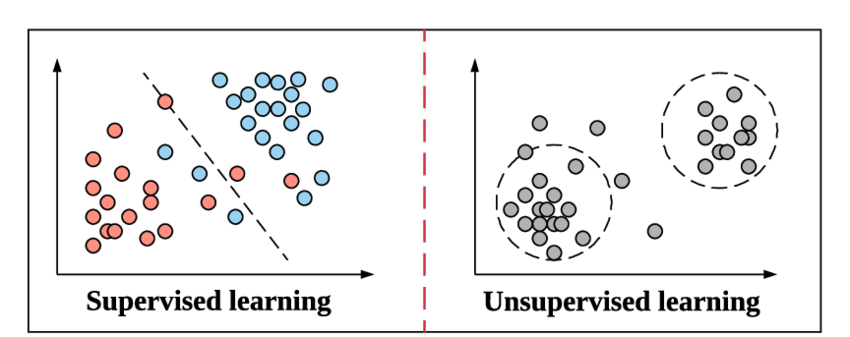
\includegraphics[height=3cm]{images/unsupervised.png}}

  \vspace*{0.5cm}

  An unsupervised learning problem consists of:
  \begin{itemize}
	\item A domain set $\mathcal{X}=\mathcal{X}^1\times\cdots\times\mathcal{X}^d$
	\item An {\color{red} unknown} probability distribution $\mathcal{D}$ on $\mathcal{X}$
	\item An {\color{blue} unlabelled} training set $S=(x_1,\ldots,x_m)$ {\color{blue} sampled} from $\mathcal{D}$
  \end{itemize}
  The aim is to find {\color{green} structure} in the data
\end{frame}

\begin{frame}
  \frametitle{Clustering}
  \centerline{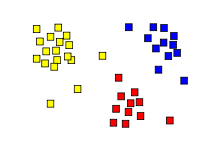
\includegraphics[height=4cm]{images/cluster.png}}
  \begin{itemize}
    \item Group sets of similar objects into {\color{red} clusters}
	\item Requires a metric that measures {\color{green} distances} between inputs
	\item Used for {\color{blue} classification}: new inputs are assigned to clusters
  \end{itemize}
\end{frame}

\begin{frame}
  \frametitle{Advantages}
  \begin{itemize}
    \item Most commonly used technique for unsupervised learning
	\item Can help find general patterns in complex data
	\item Every feature taken into account
  \end{itemize}
\end{frame}

\begin{frame}
  \frametitle{Disadvantages}
  \begin{itemize}
    \item Difficult to define precisely what is meant by ``cluster''
    \item Difficult to determine how many clusters are needed
	\item Algorithms have many parameters that have to be fine-tuned
    \item Data points might not be easily separable
  \end{itemize}
  \centerline{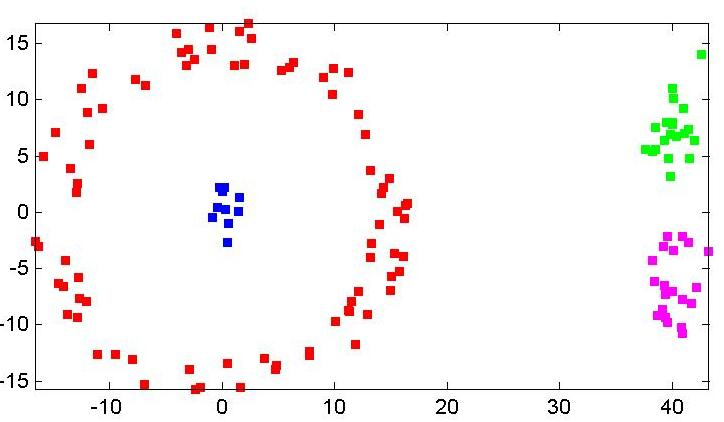
\includegraphics[height=3cm]{images/difficult2.jpg}}
\end{frame}

\begin{frame}
  \frametitle{Cluster definitions}
  \begin{itemize}
	\item Common definitions of clusters:
  \begin{itemize}
    \item Small distances between cluster members
	\item Particular intervals or statistical distributions
	\item Dense areas of the state space
  \end{itemize}
	\item Clustering can be viewed as a multi-objective optimization problem
  \end{itemize}
\end{frame}

\begin{frame}
  \frametitle{Types of clustering algorithms}
  \begin{itemize}
	\item {\bf Hierarchical}: minimize the {\color{red} distance} between the objects of a cluster
	\item {\bf Centroid-based}: minimize the distance between objects and cluster {\color{red} centroids}
	\item {\bf Distribution-based}: maximize the likelihood that the objects of a cluster belong to the same
		{\color{red} distribution}
	\item {\bf Density-based}: clusters are areas of higher {\color{red} density}
  \end{itemize}
\end{frame}

\begin{comment}
\begin{frame}
  \frametitle{Recent trends}
  \begin{itemize}
	\item Data sets tend to be larger and larger
	\item Computational performance more important than semantic meaning of clusters
	\item {\color{red} Canopy clustering}: quickly compute a rough partition of the data, and
		refine using other clustering algorithms
  \end{itemize}
\end{frame}
\end{comment}

\begin{frame}
  \frametitle{Applications}
  \begin{itemize}
    \item Pattern recognition
	\item Computer vision
	\item Marketing
	\item Information retrieval
	\item Bioinformatics
	\item Outlier detection
  \end{itemize}
\end{frame}

\section{The $k$-means algorithm}

\begin{frame}
  \frametitle{The $k$-means algorithm}
  \begin{itemize}
    \item Also known as Lloyd's algorithm
    \item Centroid-based algorithm
	\item Arguably the most popular clustering algorithm
	\item $k$: number of desired clusters
	\item Assumes {\color{red} distance metric} $d:\mathcal{X}\times\mathcal{X}\rightarrow\mathbb{R}$
	\begin{itemize}
	\item $d(x,x) = 0 \hspace*{1.1cm} \forall x\in\mathcal{X}$
	\item $d(x,y) \geq 0 \hspace*{1.1cm} \forall (x,y) \in \mathcal{X} \times \mathcal{X}$
	\item $d(x,y) = d(y,x) \hspace*{.3cm} \forall (x,y) \in \mathcal{X} \times \mathcal{X}$
	\end{itemize}
  \end{itemize}
\end{frame}

\begin{frame}
  \frametitle{Minimization problem}
  \begin{itemize}
	\item Given a {\color{red} partition} $C_1,\ldots,C_k$ of $S$, the $k$-means cost is
	\[G_{k-\text{means}}(C_1,\ldots,C_k) = \sum_{i=1}^k\sum_{x\in C_i} d(x,\mu(C_i))^2,\]
	where $\mu(C_i)$ is the {\color{blue} centroid} of subset $C_i$:
	\[\mu(C_i) = \arg\min_{\mu'\in\mathcal{X}} \sum_{x\in C_i} d(x,\mu')^2\]
	\item An optimal clustering is the solution to the minimization problem
	\[\arg\min_{C_1,\ldots,C_k} G_{k-\text{means}}(C_1,\ldots,C_k)\]
	\item {\color{red} Problem}: NP-hard to minimize
  \end{itemize}
\end{frame}

\begin{frame}
  \frametitle{Algorithm}
  \begin{block}{$k$-means clustering}
  \begin{enumerate}
    \item Input: training set $S=(x_1,\ldots,x_m)$, integer $k$
	\item Randomly choose $k$ points as centroids
	\item Repeat until convergence:
  \begin{itemize}
    \item Recompute clusters $C_1,\ldots,C_k$ given the centroids
	\item Recompute centroids $\mu_1,\ldots,\mu_k$ given the clusters
  \end{itemize}
  \end{enumerate}
  \end{block}
\end{frame}

\begin{frame}
  \frametitle{Clusters and centroids}
  \begin{itemize}
	\item Given centroids $\mu_1,\ldots,\mu_k$, each cluster $C_i$ is computed as
	\[C_i =  \left\{x\in S: i = \arg\min_{j=1}^k \left\{ d(x,\mu_j)^2 \right\} \right\}\]
	\pause
    \item Given clusters $C_1,\ldots,C_k$, each centroid $\mu_i$ is computed as
	\[\mu_i = \mu(C_i) = \arg\min_{\mu'\in\mathcal{X}} \sum_{x\in C_i} d(x,\mu')^2\]
	\pause
	\item In {\color{red} Euclidean space} ($d(x,y)=\lVert x - y \rVert$), the centroid is given by
	\[\mu_i = \mu(C_i) = \frac 1 {|C_i|} \sum_{x\in C_i} x\]
  \end{itemize}
\end{frame}

\begin{frame}
  \frametitle{Example}
  \begin{pspicture}(11,6)
	\psaxes[dx=.6,dy=.6](3,0)(9.01,6.01)
	\pscircle[fillstyle=solid,fillcolor=black](4.2,6){.07}
	\pscircle[fillstyle=solid,fillcolor=black](5.4,5.4){.07}
	\pscircle[fillstyle=solid,fillcolor=black](6,4.8){.07}
	\pscircle[fillstyle=solid,fillcolor=black](4.2,3){.07}
	\pscircle[fillstyle=solid,fillcolor=black](3.6,1.2){.07}
	\pscircle[fillstyle=solid,fillcolor=black](6.6,2.4){.07}
	\pscircle[fillstyle=solid,fillcolor=black](7.2,3){.07}
	\pscircle[fillstyle=solid,fillcolor=black](7.8,2.4){.07}
  \end{pspicture}
\end{frame}

\begin{frame}
  \frametitle{Example}
  \begin{pspicture}(11,6)
	\psaxes[dx=.6,dy=.6](3,0)(9.01,6.01)
	\psdots[dotstyle=+,dotscale=2 2,linecolor=red](4.2,6)
	\psdots[dotstyle=+,dotscale=2 2,linecolor=green](3.6,1.2)
	\psdots[dotstyle=+,dotscale=2 2,linecolor=blue](6,4.8)
	\pscircle[fillstyle=solid,fillcolor=red,linecolor=red](4.2,6){.07}
	\pscircle[fillstyle=solid,fillcolor=black](5.4,5.4){.07}
	\pscircle[fillstyle=solid,fillcolor=blue,linecolor=blue](6,4.8){.07}
	\pscircle[fillstyle=solid,fillcolor=black](4.2,3){.07}
	\pscircle[fillstyle=solid,fillcolor=green,linecolor=green](3.6,1.2){.07}
	\pscircle[fillstyle=solid,fillcolor=black](6.6,2.4){.07}
	\pscircle[fillstyle=solid,fillcolor=black](7.2,3){.07}
	\pscircle[fillstyle=solid,fillcolor=black](7.8,2.4){.07}
  \end{pspicture}
\end{frame}

\begin{frame}
  \frametitle{Example}
  \begin{pspicture}(11,6)
	\psaxes[dx=.6,dy=.6](3,0)(9.01,6.01)
	\psdots[dotstyle=+,dotscale=2 2,linecolor=red](4.2,6)
	\psdots[dotstyle=+,dotscale=2 2,linecolor=green](3.6,1.2)
	\psdots[dotstyle=+,dotscale=2 2,linecolor=blue](6,4.8)
	\pscircle[fillstyle=solid,fillcolor=red,linecolor=red](4.2,6){.07}
	\pscircle[fillstyle=solid,fillcolor=blue,linecolor=blue](5.4,5.4){.07}
	\pscircle[fillstyle=solid,fillcolor=blue,linecolor=blue](6,4.8){.07}
	\pscircle[fillstyle=solid,fillcolor=green,linecolor=green](4.2,3){.07}
	\pscircle[fillstyle=solid,fillcolor=green,linecolor=green](3.6,1.2){.07}
	\pscircle[fillstyle=solid,fillcolor=blue,linecolor=blue](6.6,2.4){.07}
	\pscircle[fillstyle=solid,fillcolor=blue,linecolor=blue](7.2,3){.07}
	\pscircle[fillstyle=solid,fillcolor=blue,linecolor=blue](7.8,2.4){.07}
  \end{pspicture}
\end{frame}

\begin{frame}
  \frametitle{Example}
  \begin{pspicture}(11,6)
	\psaxes[dx=.6,dy=.6](3,0)(9.01,6.01)
	\psdots[dotstyle=+,dotscale=2 2,linecolor=red](4.2,6)
	\psdots[dotstyle=+,dotscale=2 2,linecolor=green](3.9,2.1)
	\psdots[dotstyle=+,dotscale=2 2,linecolor=blue](6.6,3.6)
	\pscircle[fillstyle=solid,fillcolor=red,linecolor=red](4.2,6){.07}
	\pscircle[fillstyle=solid,fillcolor=blue,linecolor=blue](5.4,5.4){.07}
	\pscircle[fillstyle=solid,fillcolor=blue,linecolor=blue](6,4.8){.07}
	\pscircle[fillstyle=solid,fillcolor=green,linecolor=green](4.2,3){.07}
	\pscircle[fillstyle=solid,fillcolor=green,linecolor=green](3.6,1.2){.07}
	\pscircle[fillstyle=solid,fillcolor=blue,linecolor=blue](6.6,2.4){.07}
	\pscircle[fillstyle=solid,fillcolor=blue,linecolor=blue](7.2,3){.07}
	\pscircle[fillstyle=solid,fillcolor=blue,linecolor=blue](7.8,2.4){.07}
  \end{pspicture}
\end{frame}

\begin{frame}
  \frametitle{Example}
  \begin{pspicture}(11,6)
	\psaxes[dx=.6,dy=.6](3,0)(9.01,6.01)
	\psdots[dotstyle=+,dotscale=2 2,linecolor=red](4.2,6)
	\psdots[dotstyle=+,dotscale=2 2,linecolor=green](3.9,2.1)
	\psdots[dotstyle=+,dotscale=2 2,linecolor=blue](6.6,3.6)
	\pscircle[fillstyle=solid,fillcolor=red,linecolor=red](4.2,6){.07}
	\pscircle[fillstyle=solid,fillcolor=red,linecolor=red](5.4,5.4){.07}
	\pscircle[fillstyle=solid,fillcolor=blue,linecolor=blue](6,4.8){.07}
	\pscircle[fillstyle=solid,fillcolor=green,linecolor=green](4.2,3){.07}
	\pscircle[fillstyle=solid,fillcolor=green,linecolor=green](3.6,1.2){.07}
	\pscircle[fillstyle=solid,fillcolor=blue,linecolor=blue](6.6,2.4){.07}
	\pscircle[fillstyle=solid,fillcolor=blue,linecolor=blue](7.2,3){.07}
	\pscircle[fillstyle=solid,fillcolor=blue,linecolor=blue](7.8,2.4){.07}
  \end{pspicture}
\end{frame}

\begin{frame}
  \frametitle{Example}
  \begin{pspicture}(11,6)
	\psaxes[dx=.6,dy=.6](3,0)(9.01,6.01)
	\psdots[dotstyle=+,dotscale=2 2,linecolor=red](4.8,5.7)
	\psdots[dotstyle=+,dotscale=2 2,linecolor=green](3.9,2.1)
	\psdots[dotstyle=+,dotscale=2 2,linecolor=blue](6.9,3.3)
	\pscircle[fillstyle=solid,fillcolor=red,linecolor=red](4.2,6){.07}
	\pscircle[fillstyle=solid,fillcolor=red,linecolor=red](5.4,5.4){.07}
	\pscircle[fillstyle=solid,fillcolor=blue,linecolor=blue](6,4.8){.07}
	\pscircle[fillstyle=solid,fillcolor=green,linecolor=green](4.2,3){.07}
	\pscircle[fillstyle=solid,fillcolor=green,linecolor=green](3.6,1.2){.07}
	\pscircle[fillstyle=solid,fillcolor=blue,linecolor=blue](6.6,2.4){.07}
	\pscircle[fillstyle=solid,fillcolor=blue,linecolor=blue](7.2,3){.07}
	\pscircle[fillstyle=solid,fillcolor=blue,linecolor=blue](7.8,2.4){.07}
  \end{pspicture}
\end{frame}

\begin{frame}
  \frametitle{Example}
  \begin{pspicture}(11,6)
	\psaxes[dx=.6,dy=.6](3,0)(9.01,6.01)
	\psdots[dotstyle=+,dotscale=2 2,linecolor=red](4.8,5.7)
	\psdots[dotstyle=+,dotscale=2 2,linecolor=green](3.9,2.1)
	\psdots[dotstyle=+,dotscale=2 2,linecolor=blue](6.9,3.3)
	\pscircle[fillstyle=solid,fillcolor=red,linecolor=red](4.2,6){.07}
	\pscircle[fillstyle=solid,fillcolor=red,linecolor=red](5.4,5.4){.07}
	\pscircle[fillstyle=solid,fillcolor=red,linecolor=red](6,4.8){.07}
	\pscircle[fillstyle=solid,fillcolor=green,linecolor=green](4.2,3){.07}
	\pscircle[fillstyle=solid,fillcolor=green,linecolor=green](3.6,1.2){.07}
	\pscircle[fillstyle=solid,fillcolor=blue,linecolor=blue](6.6,2.4){.07}
	\pscircle[fillstyle=solid,fillcolor=blue,linecolor=blue](7.2,3){.07}
	\pscircle[fillstyle=solid,fillcolor=blue,linecolor=blue](7.8,2.4){.07}
  \end{pspicture}
\end{frame}

\begin{frame}
  \frametitle{Example}
  \begin{pspicture}(11,6)
	\psaxes[dx=.6,dy=.6](3,0)(9.01,6.01)
	\psdots[dotstyle=+,dotscale=2 2,linecolor=red](5.1,5.4)
	\psdots[dotstyle=+,dotscale=2 2,linecolor=green](3.9,2.1)
	\psdots[dotstyle=+,dotscale=2 2,linecolor=blue](7.2,2.6)
	\pscircle[fillstyle=solid,fillcolor=red,linecolor=red](4.2,6){.07}
	\pscircle[fillstyle=solid,fillcolor=red,linecolor=red](5.4,5.4){.07}
	\pscircle[fillstyle=solid,fillcolor=red,linecolor=red](6,4.8){.07}
	\pscircle[fillstyle=solid,fillcolor=green,linecolor=green](4.2,3){.07}
	\pscircle[fillstyle=solid,fillcolor=green,linecolor=green](3.6,1.2){.07}
	\pscircle[fillstyle=solid,fillcolor=blue,linecolor=blue](6.6,2.4){.07}
	\pscircle[fillstyle=solid,fillcolor=blue,linecolor=blue](7.2,3){.07}
	\pscircle[fillstyle=solid,fillcolor=blue,linecolor=blue](7.8,2.4){.07}
  \end{pspicture}
\end{frame}

\begin{frame}
  \frametitle{Properties}
  \begin{itemize}
    \item Greedy algorithm
    \item Very fast compared to other clustering algorithms
    \item Tends to find clusters of comparable extent
	\item Resulting regions are {\color{red} Voronoi cells}
	\item Expectation-maximization (interleaves assignment and update step)
  \end{itemize}
\end{frame}

\begin{frame}
  \frametitle{Voronoi cells}
  \centerline{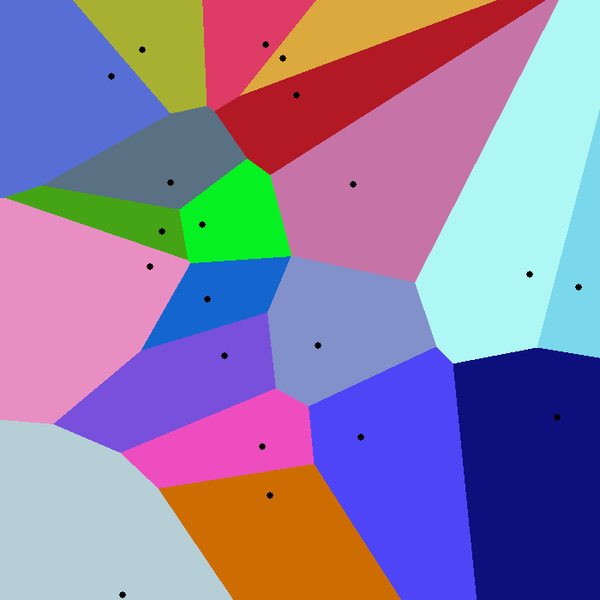
\includegraphics[height=5cm]{images/voronoi.png}}
\end{frame}

\begin{frame}
  \frametitle{Disadvantages}
  \begin{itemize}
    \item Highly dependent on the choice of $k$
    \item Highly dependent on the choice of initial centroids
	\item Cannot find clusters with more complicated shapes
	\item No guarantees on the magnitude of error (compared to optimal)
	\item Resulting cluster may not even be a local minimum
  \end{itemize}
\end{frame}

\begin{frame}
  \frametitle{Variants}
  \begin{itemize}
    \item Random restarts (different choice of initial centroids)
	\item Random partition (assign an initial cluster to each data point)
	\item $k$-medoids: arbitrary distance functions
	\item $G$-means: automatic choice of $k$
  \end{itemize}
\end{frame}

\section{Gaussian mixture models}

\begin{frame}
  \frametitle{Gaussian mixture models}
  \begin{itemize}
    \item Distribution-based algorithm
	\item Each cluster is a Gaussian distribution
	\item Compute the {\color{red} likelihood} of belonging to each cluster
	\item Data point assigned to most likely cluster
  \end{itemize}
\end{frame}

\begin{frame}
  \frametitle{Soft clustering}
  \begin{itemize}
    \item Each data point does not belong exclusively to one cluster
	\item Track the {\color{blue} likelihood} of belonging to each cluster
	\item The likelihood indicates the strength of the association between the data point and the cluster
  \end{itemize}
\end{frame}

\begin{frame}
  \frametitle{Algorithm}
  \begin{itemize}
    \item Start with $k$ random Gaussian distributions (the clusters)
	\item Expectation-maximization algorithm:
  \begin{itemize}
    \item Expectation: compute the likelihood of each data point belonging to each cluster
	\item Maximization: optimize the parameters of the Gaussians to better fit the data
  \end{itemize}
	\item Run until convergence
  \end{itemize}
\end{frame}

\begin{frame}
  \frametitle{Example}
  \centerline{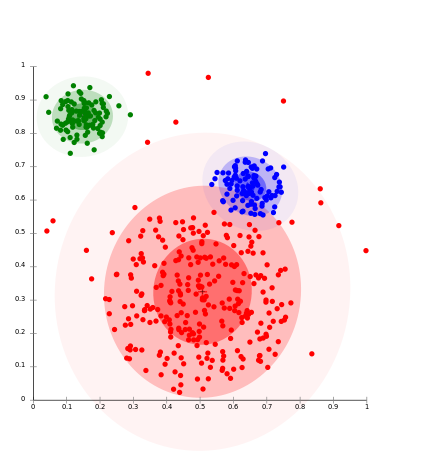
\includegraphics[height=6cm]{images/clustery.png}}
\end{frame}

\begin{frame}
  \frametitle{Disadvantages}
  \begin{itemize}
    \item Difficult to model density-based clusters
  \end{itemize}
  \centerline{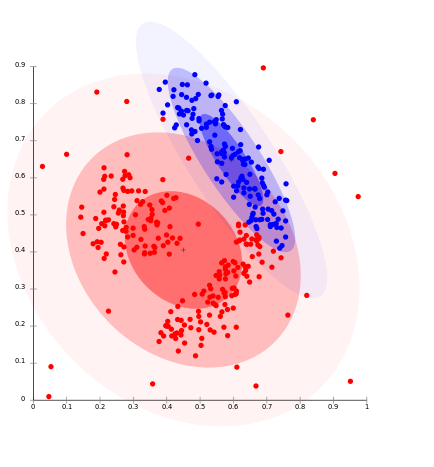
\includegraphics[height=5cm]{images/density.png}}
\end{frame}

\begin{frame}
  \frametitle{Example in one dimension}
  \centerline{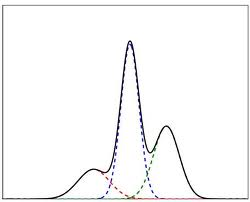
\includegraphics[height=6cm]{images/gaussian.jpg}}
\end{frame}

\section{Dimensionality reduction}

\begin{frame}
  \frametitle{High-dimensional data}
  \begin{itemize}
	\item Distance functions more costly to compute
	\item Adverse effect on performance
	\item Techniques for reduce the dimensionality of the data:
  \begin{itemize}
	\item Principal components analysis (PCA)
	\item Manifold learning
	\item Subspace clustering: focus on a subset of attributes
  \end{itemize}
  \end{itemize}
\end{frame}

\begin{frame}
  \frametitle{Principal components analysis}
  \begin{itemize}
	\item Mathematical procedure for orthogonal transformation
	\item {\color{red} Principal components}: linearly uncorrelated variables that best describe the data
	\item Resulting dimension $d'$ less than or equal to original $d$
  \end{itemize}
\end{frame}

\begin{frame}
  \frametitle{Idea}
  \begin{itemize}
	\item First principal component: direction with the largest {\color{red} variance},
		accounting for as much of the variability as possible
	\item Repeat under the constraint of orthogonality
	\item Resulting principal components describe a new coordinate system
  \end{itemize}
\end{frame}

\begin{frame}
  \frametitle{Input}
  \begin{itemize}
	\item Input: training set $S=(x_1,\ldots,x_m)$
	\item $X$: $m\times d$ data matrix with {\color{red} zero empirical mean}
	\[X = \left( \begin{array}{ccc} \textrm{-----} & (x_1 - \mu)^\top & \textrm{-----} \\ \textrm{-----} & (x_2 - \mu)^\top & \textrm{-----} \\ & \vdots & \\ \textrm{-----} & (x_m - \mu)^\top & \textrm{-----} \end{array} \right)\]
	\item $\mu = \frac 1 m \sum_{i=1}^m x_i$: {\color{red} mean} input vector
  \end{itemize}
\end{frame}

\begin{frame}
  \frametitle{Spectral decomposition}
  \begin{itemize}
	\item Given an $n\times n$ square matrix $A$, consider the linear equation
	\[Av = \lambda v\]
	\vspace*{-0.5cm}
	\pause
	\item In general, this equation has {\color{red} multiple solutions} $(\lambda_i,v_i)$
	\begin{itemize}
	\item $\lambda_i$: {\color{red} eigenvalue}
	\item $v_i$: {\color{red} eigenvector}
	\end{itemize}
	\pause
	\item If $A$ has $n$ {\color{red} linearly independent} eigenvectors, we can write
	\[A = Q \Lambda Q^{-1}\]
	\vspace*{-0.5cm}
	\begin{itemize}
	\item $Q$: $n\times n$ matrix whose columns are the eigenvectors
	\item $\Lambda$: $n\times n$ diagonal matrix whose elements are the eigenvalues
	\end{itemize}
  \end{itemize}
\end{frame}

\begin{frame}
  \frametitle{Dimensionality reduction}
  \begin{itemize}
	\item We can reduce the dimensionality using a {\color{red} linear} mapping:
	\[\tilde{x} = Wx\]
	$W$: $d'\times d$ matrix
	\pause
	\item Intuitively, $W$ should preserve as much information as possible
	\item We can formulate this as an optimization problem:
	\[\arg\min_{W,U} \sum_{i=1}^m \lVert x_i - UWx_i\rVert^2\]
	$U$: $d\times d'$ {\color{red} reconstruction matrix}
  \end{itemize}
\end{frame}

\begin{frame}
  \frametitle{Dimensionality reduction}
  \begin{itemize}
	\item For any solution to the optimization problem, $W=U^\top$:
	\[\arg\min_U \sum_{i=1}^m \lVert x_i - UU^\top x_i\rVert^2\]
	\pause
	\item {\color{red} Analytical solution}: columns of $U$ $=$ $d'$ eigenvectors of $X^\top X$ with largest eigenvalues
	\item $X^\top X$ is {\color{red} positive semidefinite}: eigenvalues satisfy
	\[\lambda_1 \geq \lambda_2 \geq \cdots \geq \lambda_n \geq 0\]
  \end{itemize}
\end{frame}

\begin{frame}
  \frametitle{Algorithm}
  \begin{block}{Principal components analysis}
  \begin{enumerate}
	\item Form the matrices $X$ and $X^\top X$
	\item Perform a spectral decomposition of $X^\top X$ to find pairs $(\lambda_i,v_i)$
	\item Sort the pairs $(\lambda_i,v_i)$ from largest to smallest eigenvalue $\lambda_i$
	\item Construct matrix $U$ whose columns are eigenvectors $v_1,\ldots,v_{d'}$
	\item The dimensionality reduction mapping is given by $\tilde{x} = U^\top x$
  \end{enumerate}
  \end{block}
\end{frame}

\begin{frame}
  \frametitle{Example}
  \centerline{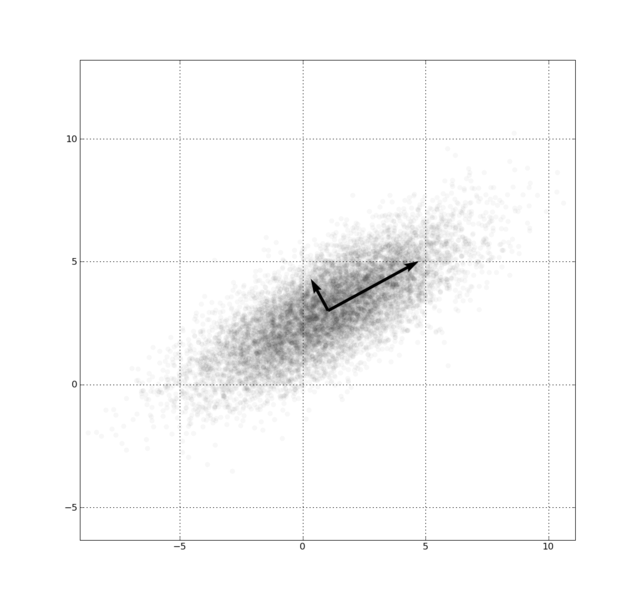
\includegraphics[height=6cm]{images/pca.png}}
\end{frame}

\begin{frame}
  \frametitle{Properties}
  \begin{itemize}
	\item Form of linear transformation
	\item Sensitive to the {\color{red} scaling} of the original variables
	\item Principal components guaranteed to be independent if the data set is
		jointly normally distributed
  \end{itemize}
\end{frame}

\begin{frame}
  \frametitle{Alternative algorithm}
  \begin{itemize}
	\item The time complexity of PCA is $O(d^3 + md^2)$
	\item In case $m \ll d$, we can perform spectral decomposition of $XX^\top$
	\item $(\lambda_i,w_i)$ solution to $XX^\top w_i=\lambda_iw_i$\\
	 $\Leftrightarrow$ $\left(\lambda_i,\frac {X^\top w_i} {\lVert X^\top w_i\rVert}\right)$ solution to $X^\top X v_i=\lambda_iv_i$ for $v_i=\frac {X^\top w_i} {\lVert X^\top w_i\rVert}$
	\item Hence mapping $U^\top$ induced by spectral decomposition of $XX^\top$!
	\item The alternative time complexity is $O(m^3 + m^2d)$
  \end{itemize}
\end{frame}

\begin{frame}
  \frametitle{Manifold learning}
  \begin{itemize}
	\item Non-linear dimensionality reduction
	\item Produce new coordinate system capturing structure in data
  \end{itemize}
  \centerline{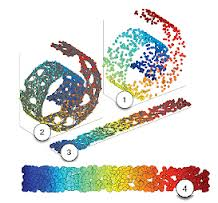
\includegraphics[height=4cm]{images/manifold.jpeg}}
\end{frame}

\begin{frame}
  \frametitle{Algorithms}
  \begin{itemize}
	\item Sammon mapping: preserve structure of inter-point distances
	\item Self-organizing maps: preserve topological properties of data
	\item Kernel principal components analysis: extension of PCA using
		kernel methods
	\item Isomap: combines Floyd-Warshall with multidimensional scaling
	\item A large variety of other algorithms exist
  \end{itemize}
\end{frame}

\section{Exercises}

\begin{frame}
  \frametitle{$k$-means}
  \begin{block}{$k$-means clustering}
  \begin{enumerate}
    \item Input: $S=(x_1,\ldots,x_m)$
	\item Randomly choose $k$ points as centroids
	\item Repeat until convergence:
  \begin{itemize}
    \item Recompute clusters $C_1,\ldots,C_k$ given the centroids
	\item Recompute centroids $\mu_1,\ldots,\mu_k$ given the clusters
  \end{itemize}
  \end{enumerate}
  \end{block}
  Show that each iteration does not increase the $k$-means cost
\end{frame}

\begin{frame}
  \frametitle{$k$-means}
  \begin{itemize}
	\item Recall that the $k$-means cost is
	\[G_{k-\text{means}}(C_1,\ldots,C_k) = \sum_{i=1}^k\sum_{x\in C_i} d(x,\mu(C_i))^2\]
	\pause
	\item Note that we can rewrite this as
	\[G_{k-\text{means}}(C_1,\ldots,C_k) = \sum_{x\in S} d(x,\mu(C(x)))^2,\]
	where $C(x)\in\{C_1,\ldots,C_k\}$ is the cluster to which $x$ belongs
  \end{itemize}
\end{frame}

\begin{frame}
  \frametitle{$k$-means}
  \begin{itemize}
	\item Given centroids $\mu_1,\ldots,\mu_k$, each cluster is recomputed as
	\[C_i' =  \left\{x\in S: i = \arg\min_{j=1}^k \left\{ d(x,\mu_j)^2 \right\} \right\}\]
	\pause
	\item Hence for each $x\in S$, it holds that
	\[d(x,\mu(C'(x)))^2 \leq d(x,\mu(C(x)))^2\]
	$C'(x)\in\{C_1',\ldots,C_k'\}$: {\color{red} new} cluster to which $x$ belongs\\
	$\mu(C_i')=\mu(C_i)=\mu_i$: {\color{red} old} centroid of $C_i$, $\forall i$
  \end{itemize}
\end{frame}

\begin{frame}
  \frametitle{$k$-means}
  \begin{itemize}
    \item Given clusters $C_1',\ldots,C_k'$, each centroid $\mu_i'$ is recomputed as
	\[\mu_i' = \arg\min_{\mu'\in\mathcal{X}} \sum_{x\in C_i'} d(x,\mu')^2\]
	\pause
	\item Hence for each $C_i'$, it holds that
	\[\sum_{x\in C_i'} d(x,\mu_i')^2 \leq \sum_{x\in C_i'} d(x,\mu_i)^2\]
  \end{itemize}
\end{frame}

\begin{frame}
  \frametitle{$k$-means}
  Putting everything together, it follows that
  \[
  \begin{cases}
  \begin{aligned}
  \action<+->{G_{k-\text{means}}(C_1',\ldots,C_k') &= \sum_{i=1}^k\sum_{x\in C_i'} d(x,\mu'(C_i'))^2 = \sum_{i=1}^k {\color{red} \sum_{x\in C_i'} d(x,\mu_i')^2}\\}
  \action<+->{ &{\color{red} \leq} \sum_{i=1}^k {\color{red} \sum_{x\in C_i'} d(x,\mu_i)^2} = \sum_{x\in S} {\color{red} d(x,\mu(C'(x)))^2}\\}
  \action<+->{ &{\color{red} \leq} \sum_{x\in S} {\color{red} d(x,\mu(C(x)))^2} = \sum_{i=1}^k\sum_{x\in C_i} d(x,\mu(C_i))^2\\}
  \action<+->{ &= G_{k-\text{means}}(C_1,\ldots,C_k)\\}
  \end{aligned}
  \end{cases}
  \]
\end{frame}

\end{document}

